\documentclass[11pt, oneside]{article} 
\usepackage{geometry}
\geometry{letterpaper} 
\usepackage{graphicx}
	
\usepackage{amssymb}
\usepackage{amsmath}
\usepackage{parskip}
\usepackage{color}
\usepackage{hyperref}

\graphicspath{{/Users/telliott_admin/Dropbox/Tex/png/}}
% \begin{center} 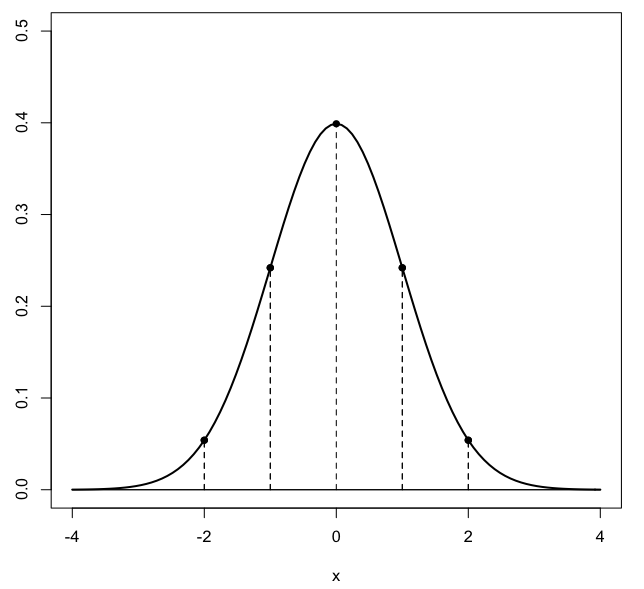
\includegraphics [scale=0.4] {gauss3.png} \end{center}

%break
\title{Volumes of revolution}
\date{}

\begin{document}
\maketitle
\Large
\label{sec:Volumes_of_revolution}

A solid of revolution is formed by revolving a curve around a central axis, typically, the $x$-axis.  We can get the volume of the solid by slicing it into disks.

In \hyperref[sec:Sphere_and_cone]{\textbf{Sphere and cone}}, we revolved a half-circle to obtain the volume of a sphere.  The integral was
\[ V = \int_{-R}^{R} \pi y^2 \ dx \]

We also did the cone:
\[ V = \pi \int_0^H ( \frac{R}{H} x)^2 \ dx \]

However, this approach can be used with any curve or pair of curves.

We also found (\hyperref[sec:Improper_integrals]{\textbf{here}}) the volume (and surface area) of Gabriel's horn, using the curve $y = 1/x$.

The volume of the solid formed by rotating the curves $f(x)$ and $g(x)$ around the $x$-axis on the interval $[a,b]$ ($f(x) < g(x)$ everywhere) is:
\[ V = \int_a^b f(x)^2 - g(x)^2 \ dx \]

For $g(x) = 0$ this resolves to the familiar form.

If the curve is given in parametric form (both $x$ and $y$ as a function of $t$), then

\[ V_x = \int_a^b \pi y^2 \ \frac{dx}{dt} \ dt \]
\[ V_y = \int_a^b \pi x^2 \ \frac{dy}{dt} \ dt \]

where $V_x$ is revolved around the $x$-axis, and so on.

The corresponding surface areas are

\[ A_x = \int_a^b 2 \pi y \ \sqrt{(\frac{dx}{dt})^2 + (\frac{dy}{dt})^2} \ dt \]
\[ A_y = \int_a^b 2 \pi x \ \sqrt{(\frac{dx}{dt})^2 + (\frac{dy}{dt})^2} \ dt \]

\subsection*{Torus}
Consider a circle of radius $R$, displaced upward from the $x$-axis.  The distance from the origin to the center of the circle is $a$.

The equation of the upper half of this circle is
\[ y = \sqrt{R^2 - x^2} + a  \]
So
\[ y^2 = R^2 - x^2 + a^2 + 2 a \sqrt{R^2 - x^2} \]

The equation of the bottom half of the circle is almost identical
\[ y  = -\sqrt{R^2 - x^2} + a  \]
So
\[ y^2 = R^2 - x^2 + a^2 - 2 a \sqrt{R^2 - x^2} \]

Subtracting the bottom from the top, the first three terms cancel and we have
\[ y_{\text{top}}^2 - y_{\text{bottom}}^2 = 4 a \sqrt{R^2 - x^2} \]
Don't forget to multiply by $\pi$:
\[ A = 4 \pi a \sqrt{R^2 - x^2} \]

Adding up the area of each slice of the donut
\[ V = \int_{-R}^{R} 4 \pi a \sqrt{R^2 - x^2} \ dx \]

We need a trig substitution:
\[ x = R \sin t \]
\[ dx = R \cos t \ dt \]
\[ \sqrt{R^2 - x^2} = R \cos t \]
So the integral is $4 \pi a$ times
\[ R^2 \int \cos^2 t \ dt \]

As always:
\[ \int \cos^2 t \ dt = \frac{1}{2} \ [ t + \sin t \cos t \ ]  \]
And if the bounds are right, that second term will disappear.  Let's see.
\[ x = [-R,R] \]
\[ t = [-\pi/2,\pi/2] \]
The second term does go away, giving $\pi$ for what's in the brackets, and we obtain finally
\[ V = 4 \pi a \cdot R^2 \cdot \frac{\pi}{2} \]
\[ = 2 \pi a \cdot \pi R^2 \]

This is the same as obtained by multiplying the area of the cross-section of the torus by the distance traveled by the center in revolving around the $x$-axis.  The general principle is named after Pappus.

\end{document}